\documentclass[10pt,a4paper]{article}
\usepackage[utf8x]{inputenc}
\usepackage[danish]{babel}
\usepackage{amsmath}
\usepackage{mathtools}
\usepackage{framed}
\usepackage{amsfonts}
\usepackage{hyperref}
\usepackage{todonotes}
\usepackage{float}
\usepackage{amssymb}
\setlength{\parindent}{0pt}
\usepackage{graphicx}
\usepackage{fullpage}
\DeclarePairedDelimiter\ceil{\lceil}{\rceil}
\DeclarePairedDelimiter\floor{\lfloor}{\rfloor}
\newcount\colveccount
\newcommand*\colvec[1]{
        \global\colveccount#1
        \begin{pmatrix}
        \colvecnext
}
\def\colvecnext#1{
        #1
        \global\advance\colveccount-1
        \ifnum\colveccount>0
                \\
                \expandafter\colvecnext
        \else
                \end{pmatrix}
        \fi
}
\begin{document}
\section{Analysis}
Since the dataset consisting of the raw data is a contionous dataset, one have to be binned before they can be processed. Binning is a way of dicretization the data in to numerical variables into categorical counterparts. The binary data were binned based on interval sizes.  A small intervall size would create a large amount bins categories and a large intervall would create a small amount of bin category.  

First were the model created with different number of bins from a dataset consisting one person, and then tested with another dataset.

\begin{figure}[H] 
\centering
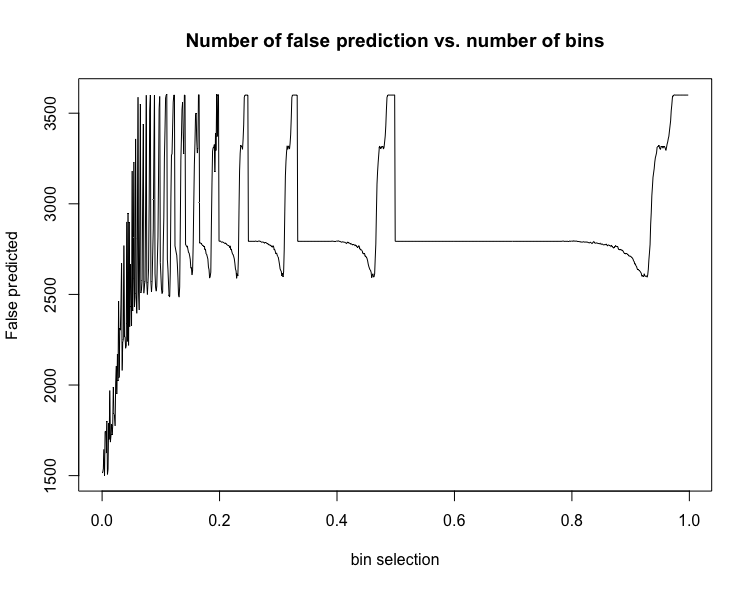
\includegraphics[width = \textwidth]{number_of_false_prediction_vs_number_of_bins_plot.png}
\label{fig:false_g_g}
\caption{Graph showing amount palse precidiction vs. interval size of the bins}
\end{figure}

Based from the figure \ref{fig:false_g_g}, could it be seen that  the amount of false prediction computed were dependent of the number of bins, which makes sense as the variabillity of the data changes, based on this observation were same test peformed for the whole class vs. one person who was not part of the complete dataset. 

\begin{figure}[H]
\centering
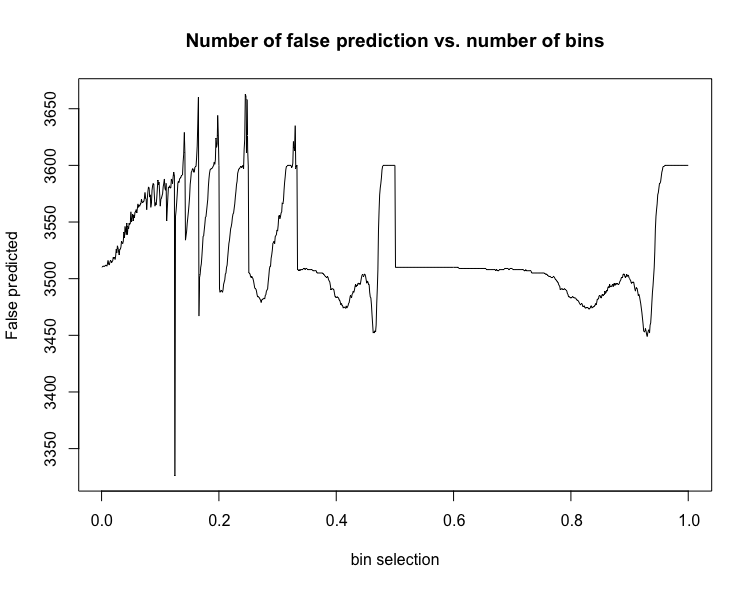
\includegraphics[width = \textwidth]{g2M2vsFewer.png}
\label{fig:false_g_f}
\caption{Graph showing amount palse precidiction vs. interval size of the bins}
\end{figure}

The dataset used for testing entailed  4000 observation, which the previous one also had but comparing the the them both shows that the result of increasing the amount of training make the prediction worse, which wasnt the case before.

Looking at the confusion matrix from the iterations shows this

\begin{figure}[!htb]
\minipage{0.32\textwidth}
  \includegraphics[width=\linewidth]{confus_10.eps}
\label{fig:awesome_image1}
\caption{bin selection - 0.010}
\endminipage\hfill
\minipage{0.32\textwidth}
  \includegraphics[width=\linewidth]{confus_32.eps}
\label{fig:awesome_image2}
\caption{bin selection - 0.032}
\endminipage\hfill
\minipage{0.32\textwidth}%
  \includegraphics[width=\linewidth]{confus_62.eps}
 \label{fig:awesome_image3}
 \caption{bin selection - 0.062}
\endminipage
\end{figure}

	
Looking at the confusion matrices  in figure \ref{fig:awesome_image1},\ref{fig:awesome_image2},\ref{fig:awesome_image3} shows that most of data set being incorrectly classified toward Class 1. 	This were not the case for one specific only, but the same occured from different members, and the false prediction rate were moving toward the same numbers as the one seen in figure \ref{fig:false_g_f}. 

A different binning method could consist of binning the dataset of dataset based on the PDF.
Which also were tried, which did shed a bit light on the issue seen before 

\begin{figure}[H]
\centering
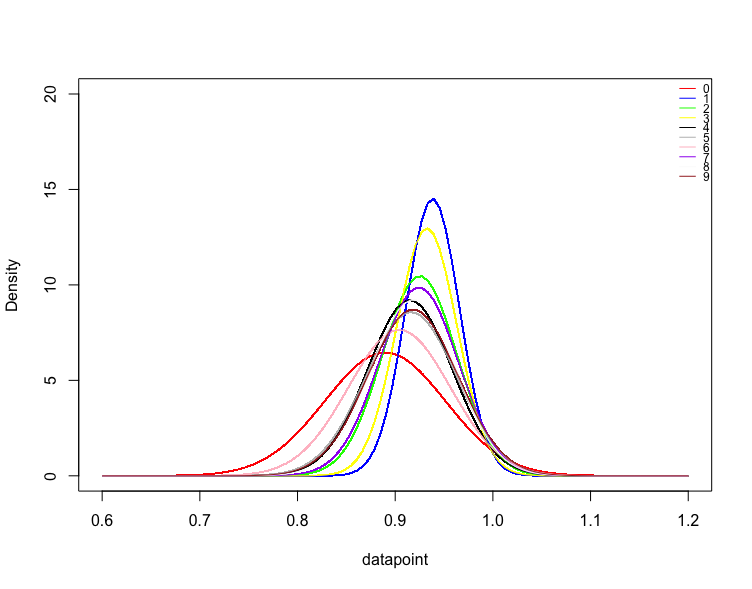
\includegraphics[width =  \textwidth]{ndist_muld_class.png}
\end{figure} 

It seems the like the space which the digit number 1 resides in has a very high density, which could explain why most of the predicition which were found went towards that value. 
Other than that, it also shows that the class is in general is pretty interlapped with each other, which indicate that the method itself might not be that suitable for this type of problem.  The method seems based from figure \ref{fig:false_g_g} better or more accurate at smaller dataset than bigger dataset. 
\end{document}